\documentclass[a4paper,12pt]{article}
\usepackage[utf8]{inputenc}

% Larger borders -- we do not want do waste paper, even if it is only paper on screen =)
\usepackage[top=2.5cm, bottom=2.5cm, left=2cm, right=2cm]{geometry}

% No paragraph indentation
\setlength{\parindent}{0cm}

% Palatino font (nicer serif font: Times is for oldies)
\renewcommand*\rmdefault{ppl}

% Nested itemize list bullet style
\renewcommand{\labelitemi}{$\bullet$}
\renewcommand{\labelitemii}{$\circ$}
\renewcommand{\labelitemiii}{--}

% Math packages
\usepackage{amsmath}
\usepackage{amsfonts}
\usepackage{amssymb}

% Graphic packages
\usepackage{graphicx}
\usepackage{float}
\usepackage{adjustbox}
\usepackage{tikz}
\usepackage{forest,array}
\usetikzlibrary{shadows}

% Timing diagrams
\usepackage{tikz-timing}
\usetikztiminglibrary{arrows}

% Graphs styles
\forestset{
  giombatree/.style={
    for tree={
      grow = east,
      parent anchor=east,
      child anchor=west,
      edge={rounded corners=2mm},
      fill=violet!5,
      drop shadow,
      l sep=10mm,
      edge path={
        \noexpand\path [draw, \forestoption{edge}] (!u.parent anchor) -- +(5mm,0) -- (.child anchor)\forestoption{edge label};
      }
    }
  }
}
\forestset{
  qtree/.style={
    for tree={
      parent anchor=south,
      child anchor=north,
      align=center,
      edge={rounded corners=2mm},
      fill=violet!5,
      drop shadow,
      l sep=10mm,
    }
  }
}

% Hides ugly links from the index
\usepackage[hidelinks]{hyperref}

% Landscape format pdf pagess
\usepackage{pdflscape}

% Overline in text mode
\makeatletter
\newcommand*{\textoverline}[1]{$\overline{\hbox{#1}}\m@th$}
\makeatother

%%%%%%%%%%%%%%%%%%%%%%%%%%%%%%%%%%%%%%%%%%%%%%%%%%%%%%%%%%%%%%%%%%%%%%%%
% Specific commands for this document
\newcommand{\computername}{CA~19.32}
\newcommand{\memoryname}{Elephant}

% Title
\title{\memoryname{} DRAM}

% Authors
\author{G. Alvaro, F. Barbarulo, D. Comola, F. Fornaini, R. Polini, G.B. Rolandi}

\begin{document}
\maketitle
\tableofcontents

\clearpage

\section{Introduction}

This document describes the working details of the main memory and the main bus of the Computer~Architecture course computer.

\subsection{Bus}
Main bus is 16~bit wide address and 32~bit wide data bus.

\subsection{\memoryname{}}
\memoryname{} is a SDR DRAM, single data rate dynamic random access memory.

It can hold a total amount of 512~Kbit (64~KiB) of data, and can be accessed as 16~K locations of 32~bit (4 B) each.

\section{Main computer bus}
Physical main bus of \computername{} presents the following wires.

\begin{figure}[H]
\centering
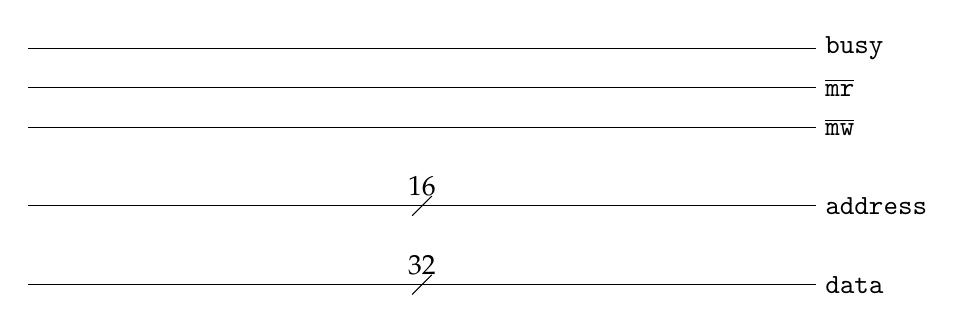
\begin{tikzpicture}
  % data wires
  \draw (0, 1)--(10, 1);
  \node at (5, 1){};
  \node [draw, strike out] at (5, 1){};
  \node [above] at (5, 1){32};
  \node [right] at (10, 1){\texttt{data}};

  % address wires
  \draw (0, 2)--(10, 2);
  \node at (5, 2){};
  \node [draw, strike out] at (5, 2){};
  \node [above] at (5, 2){16};
  \node [right] at (10, 2){\texttt{address}};

  % mw
  \draw (0, 3)--(10, 3);
  \node [right] at (10, 3){\textoverline{\texttt{mw}}};
  % mr
  \draw (0, 3.5)--(10, 3.5);
  \node [right] at (10, 3.5){\textoverline{\texttt{mr}}};

  % busy wire
  \draw (0, 4)--(10, 4);
  \node [right] at (10, 4){\texttt{busy}};
\end{tikzpicture}
\caption{main bus of \computername{}}
\end{figure}

% explanation
\begin{itemize}
  \item \textbf{busy:} this wire represents the busy status of the bus; the busy wire is active high.
  \item \textbf{\textoverline{mr}:} this wire issues a read data command, and instructs a module to put data from its internal structures onto the bus; the \textoverline{mr} wire is active low;
  \item \textbf{\textoverline{mw}:} this wire issues a write data command, and instructs a module to retrieve data from the bus and put into its internal structures; the \textoverline{mw} wire is active low;
  \item \textbf{address:} is 16~wires wide and selects the address from which/to which data must be read/written;
  \item \textbf{data:} is 32~wires wide and holds the actual data that must be read or written;
\end{itemize}

Thus, main computer bus can be represented in the simulation software by means of the following structures:

\begin{verbatim}
enum request_t { READ, WRITE };

struct bus_status {
    request_t request;
    uint16_t address;
    uint32_t data;
};

class Bus {
    private:
        bool busy;
        request_t request;
        uint16_t address;
        uint32_t data;
    public:
        Bus();
        bool set(bus_status *s);
        bool get(bus_status *s);
};
\end{verbatim}

Please note that the address line is 16~bit wide, but only 14 of them are actually used, since \memoryname{} holds only $2^{14} = 16K$ memory locations.
In particular, the 2 least significant bits are always assumed to be 0.

This choice has been agreed with the cache controller designers.

% BHA Protocol
\subsection{Bus handshake protocol}
In the simulation software, modules can:
\begin{itemize}
  \item be idle: this corresponds to the high impedance physical state;
  \item perform a read action from the bus;
  \item perform a write action on the bus;
\end{itemize}

Actions on bus must be performed in the simulation using the following protocol.

\begin{itemize}
  \item being idle: \texttt{set()} and \texttt{get()} methods of \texttt{Bus} class must not be called;
  \item read data: data can be read only upon receiving a message from another module. Data can be read using the \texttt{get()} method. It is not possible to read data more than once.
  \item write data: data can be written using the \texttt{set()} method;
  \begin{itemize}
    \item if busy bit is~1, data is not actually written onto the bus, \texttt{set()} method returns \texttt{false} and module must wait and schedule data writes onto the bus at a later time (eg. next clock tick);
    \item if busy bit is~0, data is actually written onto the bus and \texttt{set()} method returns \texttt{true}.
    Once written data to bus, destination module must be notified of the bus change by sending it a message using methods provided by the orchestrator.
    For the sake of simplicity, message passed through the orchestrator can be tought as a model for the hardware \emph{enable} wire;
  \end{itemize}
\end{itemize}

Please note that this does not model the actual hardware behavior, since a reading module can not clear a set bit on the bus;
moreover, this get/set protocol does not properly fit the event-driven programming paradigm.
But since it is not necessary to perfectly reproduce the hardware behavior, and since a perfectly event driven protocol introduces unnecessary complications, this handshake has been chosen in order to simplify the simulation software.

Note: since simulation is sequential and modules are always notified in the same order, concurrency is not actually modeled, and some modules can suffer from starvation.

% thus, a proper read/write operation can be represented in time like the following timing diagram:
% busy
% mr
% mw
% address
% data
% (be careful and remember to represent both the read and the write operation examples)

\section{DRAM Internals}
\subsection{Circuit}
A common DRAM memory is internally organized like the following circuit.

A bit at the cross of the two dashed wires has been highlighted to help understanding.

\begin{figure}[H]
\centering
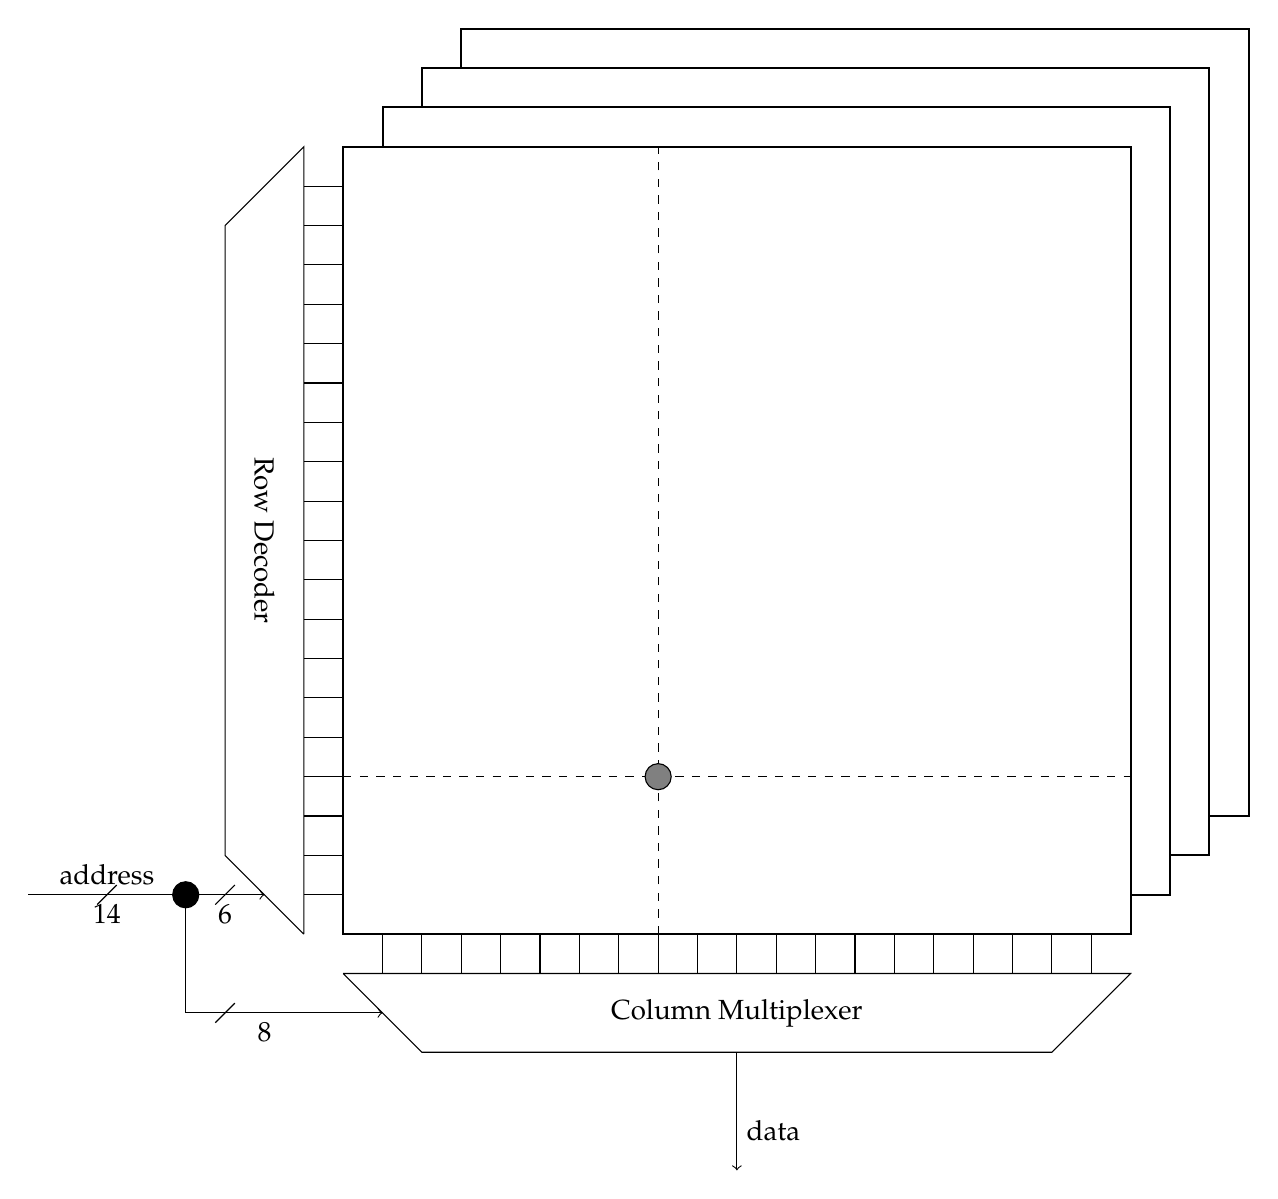
\begin{tikzpicture}
  % matrix square
  \foreach \x in {3,...,0}
    %~ \draw[line width=0.25mm] (10 + \x/2, 10 + \x/2)--(20 + \x/2, 10 + \x/2)--(20 + \x/2, 20 + \x/2)--(10 + \x/2, 20 + \x/2)--(10 + \x/2, 10 + \x/2);
    \draw[fill=white, line width=0.25mm] (10 + \x/2, 10 + \x/2) rectangle (20 + \x/2, 20 + \x/2);
  % matrix lines
  \foreach \x in {1,...,19}
    \draw (10 + \x / 2, 9.5)--(10 + \x / 2, 10);
  \foreach \x in {1,...,19}
    \draw (9.5, \x / 2 + 10)--(10, \x / 2 + 10);

  % row decoder
  \draw (9.5, 10)--(9.5, 20)--(8.5, 19)--(8.5, 11)--(9.5, 10);
  \node[rotate=270] at (9, 15){Row Decoder};

  % column multiplexer
  \draw (10, 9.5)--(20, 9.5)--(19, 8.5)--(11, 8.5)--(10, 9.5);
  \node at (15, 9){Column Multiplexer};

  % address lines
  \draw[->] (6, 10.5)--(9, 10.5);
  \draw[->] (8, 9)--(10.5, 9);
  \draw (8, 10.5)--(8, 9);

  % address lines split point
  \node[draw, circle, fill=black] at (8, 10.5){};

  % address lines width markers
  \node[draw, strike out] at (7, 10.5){};
  \node[below] at (7, 10.5){14};
  \node[above] at (7, 10.5){address};

  \node[draw, strike out] at (8.5, 10.5){};
  \node[below] at (8.5, 10.5){6};

  \node[draw, strike out] at (8.5, 9){};
  \node[below] at (9, 9){8};

  % input/output line
  \draw[->] (15, 8.5)--(15, 7);
  \node[right] at (15, 7.5){data};

  % example bit
  \draw[dashed] (10, 12)--(20, 12);
  \draw[dashed] (14, 10)--(14, 20);

  \node[draw, circle, fill=gray] at (14, 12){};

\end{tikzpicture}
\caption{Simplified DRAM internal circuit}
\end{figure}

\memoryname{} is a DRAM actually made by:
\begin{itemize}
  \item 32 matrixes: matrix \emph{n} holds the corresponding \emph{n}-th bit of the word connected to the bus;
  each matrix consists of $64 \times 256$ cells;
  each cell holds one bit;
  for practicity, in the above figure, only 4 matrixes have been drawn;
  \item a row decoder: the row decoder is controlled by the 6 most significant bits of the address, and is used to select one of the $2^{6} = 64$ rows of the matrix;
  \item a column multiplexer: the column multiplexer is controlled by the 8 least significant bits of the address, and is used to select one of the $2^{8} = 256$ columns of the matrix;
\end{itemize}

\memoryname{} is compatible with a real world DRAM, and is even simpler, since current memories have up to 64~bit wide buses and up to 8~K rows and columns.
\\
However, note that the above figure does not exactly represent a real DRAM, since some parts of the circuit, like the sense amplifier, have not been drawn because they are not relevant in our discussion.

\subsection{Input and output}
A memory controller is required to actually read and write a DRAM.
It can reside inside the CPU/cache, on an external chip on the computer main board, or inside the memory itself; its positioning and details have not been taken in account, but we must suppose it exists somewhere.

To control and actually read and write a DRAM, the following control lines are used by the memory controller.

\begin{itemize}
  \item \textbf{\textoverline{ras}}: the \emph{row address strobe} signal enables the row decoder circuit;
  \item \textbf{\textoverline{cas}}: the \emph{column address strobe} signal enables the column multiplexer circuit;
  \item \textbf{r/\textoverline{w}}: the \emph{read/write} signal controls if the cell has to be read or written;
  \item \textbf{address}: the \emph{address} line holds the memory address of the cell;
  \item \textbf{data}: the \emph{data} line holds the data read or written from/to the cell;
\end{itemize}
% all I/O lines and their description:
% /ras
% /cas
% Address
% R/W
% data

Reading and writing data in the matrix requires strict timing constraints to allow capacitors, sense amplifier and all the electronics to work properly.
Different timings can be used, as explained in the following section.

\section{DRAM control}

\subsection{Simple access}
This timing diagram represents the simplest memory cicle that can be used to read and write data in memory.

\begin{minipage}{.45\textwidth}
\begin{figure}[H]
\centering
\begin{tikztimingtable}
{\textoverline{ras}}  & H H L L L      L L L L H H\\
{\textoverline{cas}}  & H H H H L      L L H H H H\\
{r/\textoverline{w}}  & H H H H H      4H 2H\\
{addr}                & U 5D{address}  5U \\
{data}                & U 4U           4D{data} 2U\\
\end{tikztimingtable}
\caption{simple read}
\end{figure}
\end{minipage}
\begin{minipage}{.45\textwidth}
\begin{figure}[H]
\centering
\begin{tikztimingtable}
{\textoverline{ras}}  & H H L L L      L L L L H H\\
{\textoverline{cas}}  & H H H H L      L L H H H H\\
{r/\textoverline{w}}  & H H L L L      L H 4H\\
{addr}                & U 5D{address}  5U \\
{data}                & U 4U           4D{data} 2U\\
\end{tikztimingtable}
\caption{simple write}
\end{figure}
\end{minipage}

\subsection{Fast page access}
When accessing data it is possibile to take advantage of the principle of locality.

Usually programs are sequential and have small loops, thus they use to access a small region of memory for a while. Moreover, they usually make computations over the same data for a while.

To take advantage of both the spatial and the temporal locality of programs, it is possible to drive the memory matrix in such a way there is no need to make a complete full simple memory cycle for every access, but some operations can be avoided to save time.

More in details, it is not necessary to deassert the \emph{row address strobe} when memory locations are accessed sequentially and row number does not change.

Proper timing diagrams for fast page access are as the following.

\begin{minipage}{.45\textwidth}
\begin{figure}[H]
\centering
\begin{tikztimingtable}
{\textoverline{ras}}  & H H L L L      L L L L L L    L L L L L 3L 2H \\
{\textoverline{cas}}  & H H H H L      L L H H H H    H L L L H 5H\\
{r/\textoverline{w}}  & H H H H H      4H 2H          5H 5H\\
{addr}                & U 5D{address}  4U             4D{address}    7U \\
{data}                & U 4U           4D{data} 2U    U U U 4D{data} 3U\\
\end{tikztimingtable}
\caption{fast page read}
\end{figure}
\end{minipage}
\begin{minipage}{.45\textwidth}
\begin{figure}[H]
\centering
\begin{tikztimingtable}
{\textoverline{ras}}  & H H L L L      L L L L L L    L L L L L 3L 2H \\
{\textoverline{cas}}  & H H H H L      L L H H H H    H L L L H 5H\\
{r/\textoverline{w}}  & H H H H L      2L 2H 2H       2H 3L 5H\\
{addr}                & U 5D{address}  4U             4D{address}    7U \\
{data}                & U 4U           4D{data} 2U    U U U 4D{data} 3U\\
\end{tikztimingtable}
\caption{fast page write}
\end{figure}
\end{minipage}
% TODO -- missing fast page write cycle


\section{Timings definition}
% t_CL  CAS latency
% t_RCD row address to column address delay
% t_RP  row precharge time
% t_RAS number of clock cycles to refresh a row

% and their description

\section{Interesting cases}
% accessing a bit from a DRAM with the right row open (CL)
% accessing a bit from a DRAM without an active row (t_RCD + t_CL)
% accessing a bit from a DRAM with the wrong row open (t_RP + t_RCD + t_CL)

\section{Test}
% test

\section{Transfer speed}
Since this is a \emph{single data rate} memory, in short SDR, it is theoretically possible to read or write data from/to the memory once for every rising edge of the bus clock.

Thus, maximum theoretical transfer speed is given by the following formula:

$$ s_{max} =  f \cdot B_w $$

where

\bgroup
\def\arraystretch{1.5}
\begin{table}[H]
\center
\begin{tabular}{| c | c | c |}\hline
\textbf{symbol} & \textbf{unit} & \textbf{description} \\ \hline
$ s_{max} $ & $ \frac{bit}{s} $ & maximum theoretical speed \\ \hline
$ f $ & Hz & bus frequency \\ \hline
$ B_{w} $ & bit & bus width \\ \hline
\end{tabular}
\end{table}
\egroup

\section{EOF}
This is the End of File.

\end{document}
